A major goal of the thesis was to improve the performance of array-based languages like \matlab and Python's NumPy library by compiling computationally intensive functions to C++. To demonstrate these performance results, we compared the performance of the generated code with that provided by various tools for scientific computing. 17 \matlab benchmarks and 9 Python benchmarks were used to perform this comparision. Different variations of generated code that can be generated by turning optimisations on and off were also tested. 

In this chapter, we give a brief description of the benchmarks that were used to test the performance followed by the results themselves and our analysis of these results. 
\section{Benchmarks}
The \matlab benchmarks used for the performance were obtained from various sources. The sources include the FALCON project\cite{DeRose:1999} , the OTTER project \cite{quinn}, Chalmers university of technology\footnote{\url{http://www.elmagn.chalmers.se/courses/CEM/}}, Mathworks central file exchange\footnote{\url{http://www.mathworks.com/matlabcentral/fileexchange}} and the presentation on parallel programming in \matlab by Burkhadt and Cliff\footnote{\url{http://people.sc.fsu.edu/~jburkardt/presentations/matlab_parallel.pdf}}. The benchmarks cover commonly occurring \matlab features such as builtin function calls, array indexing including slicing operations and array operations like array addition, matrix multiplication, etc. Table \ref{tab:matBench} gives the list of benchmarks used along with their descriptions and source.  
% Please add the following required packages to your document preamble:
% \usepackage{graphicx}
\begin{table}[h]
\resizebox{\columnwidth}{!}{%
\centering
\begin{tabular}{|c|c|c|}
\hline
Benchmark  & Source               & Description\\
\hline 
bbai       & MATLAB file exchange & Implementation of the Babai estimation algorithm \\
\hline 
bubl       & McLab                & Bubble Sort \\
\hline 
capr       & Chalmers University  & \begin{tabular}{@{} c@{}} Computes the capacitance of a transmission line \\ using fine difference and Gauss-seidel\end{tabular} \\
\hline 
clos       & Otter project        & Calculates the transitive closure of a directed graph \\
\hline 
crni       & Falcon project       & Crank-Nicholson solution to the heat equation \\
\hline
dich       & Falcon project       & Dirichlet solution to Laplace's equation\\
\hline
fiff       & Falcon project       & Computes the finite difference solution to the wave equation \\
\hline
ldgr       &                      & Calculates derivatives of Legendre polynomials \\
\hline
mbrt       & McFor project        & Computes Mandelbrot sets \\
\hline
nb1d       & Otter project        & Simulates the 1-dimensional n-body problem \\
\hline
matmul     & McLab                & naive matrix multiplication \\
\hline
mcpi       & McLab                & Calculates $\pi$ by the Monte Carlo method   \\
\hline
numprime   & Burkardt and Cliff   & \begin{tabular}{@{} c@{}} Simulates the sieve of Eratosthenes for  \\calculating number of prime numbers less than a given number \end{tabular} \\
\hline
scra       & ACM CALGO            & \begin{tabular}{@{} c@{}} Implementation to produce a reduced-rank \\ approximation to a matrix \end{tabular}   \\
\hline
spqr       & ACM CALGO            & \begin{tabular}{@{} c@{}} Implementation to compute a pivoted \\ semi-QR decomposition of an m-by-n matrix A \end{tabular} \\
\hline
quadrature & Burkardt and Cliff   &  \begin{tabular}{@{} c@{}} Simulates the quadrature approach \\ for  calculating integral of a function \end{tabular} \\
\hline
\end{tabular}
}
\caption{List of \matlab Benchmarks used for experiments}
\label{tab:matBench}
\end{table}

Many of the Python are python ports of the Ostrich benchmark suite\cite{Khan:2014:UJW:2661088.2661090}. The benchmarks contain scalar operations as well as array index operation. 6 of the 9 Python benchmarks support parallelism. Table \ref{tab:pyBenches} gives the list of Python benchmarks that were used.    % table for python benchmarks. 
\begin{table}[h]
\centering
\begin{tabular}{|c|c|c|}
\hline
Benchmark Name & Source    & Description                                                                                                                                              \\ \hline
arc\_distance  & PyBenches &                                                                                                                                                          \\ \hline
fft            & Pydwarfs  & Fast Fourier Transform                                                                                                                                   \\ \hline
growcut        & PyBenches &  Implementation of GrowCut segmentation                                                                                                                                                         \\ \hline
julia          & PyBenches &                                                                                                                                                          \\ \hline
lud            & PyDwarfs  & \begin{tabular}[c]{@{}c@{}}LU decomposition  factors a matrix as the product of a \\ lower triangular matrix and an upper triangular matrix\end{tabular} \\ \hline
pagerank       & PyDwarfs  & PageRank is a link analysis algorithm used by Google Search                                                                                              \\ \hline
pairwise       & PyBenches &                                                                                                                                                          \\ \hline
spmv           & PyDwarfs  & Sparse Matrix-Vector Multiplication                                                                                                                      \\ \hline
srad           & PyDwarfs  & \begin{tabular}[c]{@{}c@{}}Tracks the movement of a mouse heart over a sequence  of 104\\ 609x590 ultrasound images to record response to the stimulus \end{tabular} 
\\ \hline
\end{tabular}
\caption{List of Python Benchmarks used for experiments}
\label{tab:pyBenches}
\end{table}

\section{Experimental Setup}
We ran separate experiments for \matlab and Python benchmarks. The \matlab benchmarks were executed on the Mathworks' 2014b release of \matlab. We also used the Mathworks' Matlab-coder implementation to compile the benchmarks to C++ converted to a dynamic library similar to the method used by \velocty. In case of the Python benchmarks, we used the reference C-Python interpreter version 3.2.3  and Cython\cite{cython} version 0.21, which is a compiler used to generate C-extensions for Python.

Moreover, different variations of the code generated by \velocty were also tested. These variations include C code without optimisations and without bounds checks, C code with bounds checks but without optimisations, C code with bounds check optimisations, C code with memory optimisations and C code with OpenMP pragmas. The MEX compiler was used to compile the C code generated from \matlab to a shared library that could be called from \matlab. MEX internally uses the gcc-4.6.4 compiler. We use the gcc-4.6.4 compiler through distutils for compiling the C code generated from the Python benchmarks. 

All the benchmarks were tested on a machine running GNU/Linux(3.8.0-35-generic \#52-Ubuntu) with a Intel(R) Core(TM) i7-3820 CPU @ 3.60GHz with 16GB of memory. 
\section{Results}
This section describes the experimental results that were obtained for \matlab and Python.
\subsection{\matlab Results}
We ran experiments on 17 \matlab benchmarks. We compared the C backend without bounds checks with the Mathworks' \matlab implementation and \matlab-coder. We measured the speedup of the C backend and the \matlab-coder versions compared to  Mathwork's \matlab.Figure \ref{fig:results_cwochecks} shows a bar graph with the results of the experiment. The red bars show the speedup of \matlab-coder and the blue bars show the speedup of the C backend. The geometric mean for the speedup of the C version was 6.17 as compared to the geometric mean of 3.89 for the \matlab-coder version. The largest speedup was shown by the quadrature benchmark. The benchmark was 318 times faster than Mathworks' \matlab. The benchmark consists of operations on scalar operations and hence gives a high speedup. The smallest speedup of 1.18, is given by the closure benchmark. The benchmark's computationally intensive code section is a while loop containing a matrix multiplication operation. All three versions, the C backend, Mathwork's \matlab and \matlab-coder use the Intel MKL BLAS library and hence show similiar performance. 
\begin{figure}[htbp]
\centering
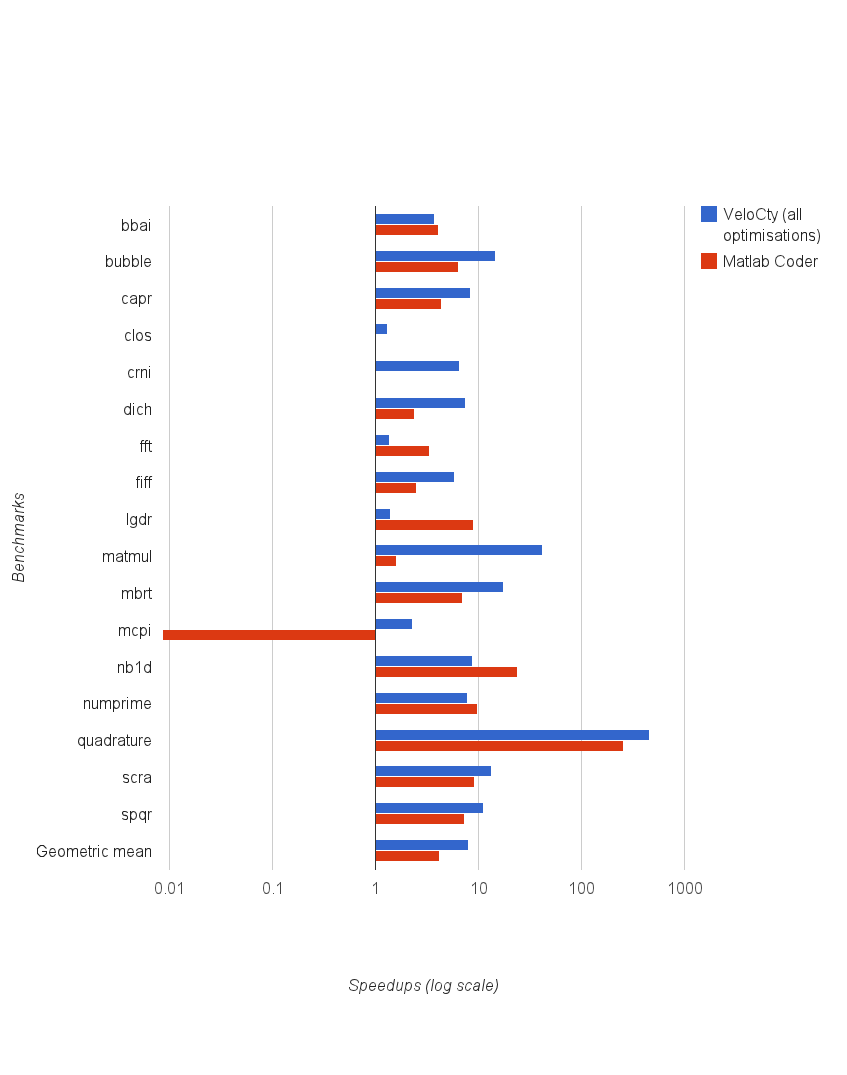
\includegraphics[scale=0.6]{Figures/results_cwochecks.png}
\caption{Experimental results for the C backend without checks}
\label{fig:results_cwochecks}
\end{figure}

For most benchmarks, our C backend was faster than \matlab-coder. The benchmarks, bbai, lgdr, nb1d, fft, scra and spqr are execptions. Bbai, scra and spqr showed poorer performance because of memory allocations from array operations performed inside a loop. Performance of these four benchmarks was improved due to the memory optimisation described in Section \ref{sec:memoptimise}. Lgdr and nb1d contain array slicing and array operations which do not internally make calls to the BLAS library and hence take longer to execute compared to \matlab-coder. The fft benchmark contains a loop whose direction can not be identified at run time and hence a loop vector needs to be initialised and iterated over as described in Subsection \ref{subsec:forStmt}. 

As we can also observe \matlab-coder is shows a positive speedup on all benchmarks except for mcpi. The reason for this is that the benchmark contains a loop with random function calls inside the body. These functions return a single scalar value. However, in case of \matlab-coder, an 1x1 matrix is returned. Since a heap allocation is needed for every iteration, the benchmark is significantly slower than Mathworks' \matlab. 

When comparing the execution times of the C backend with and without bounds checks, we observed that the execution times of benchmarks containing array slicing or array operations were not affected by turning the checks on. On the other hand, benchmarks consisting of simple indexing operations show a larger slowdown when array bounds checks were turned on. Figure \ref{fig:results_cwchecks} gives the execution times of the \matlab benchmarks for the C backend with and without bounds checks. As we can see, 6 of the 17 benchmarks show a slow down when bounds check are added. The benchmarks include fft, fiff, matmul, bubble, capr and dich. 


\begin{figure}[htbp]
\centering
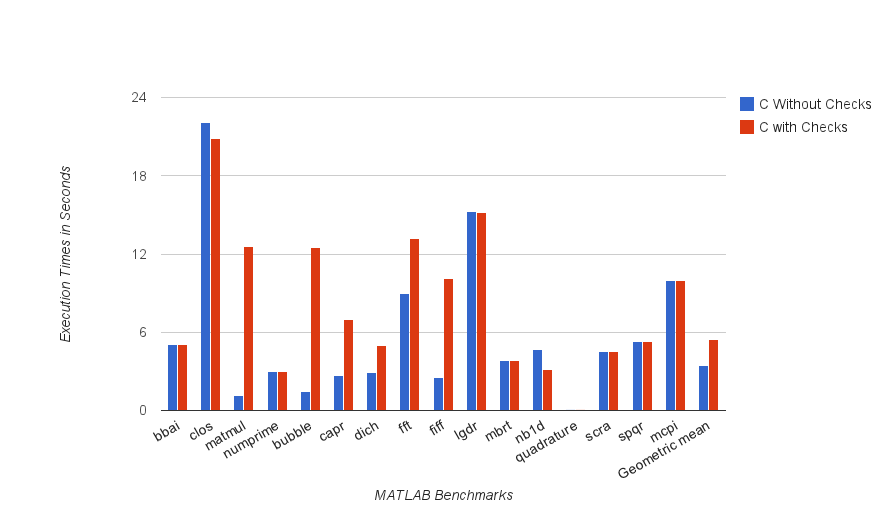
\includegraphics[scale=0.5]{Figures/results_cwchecks.png}
\caption{Comparison of the execution times of C backends with and without benchmarks. }
\label{fig:results_cwchecks}
\end{figure}
\subsection{Python Results}
We ran experiments on 9 Python benchmarks. We compared the generated C code without bounds checks to Cython and the CPython interpreter. Figure \ref{fig:results_cwochecks_py} is a bar graph showing the speedup of the generated C code and the Cython code compared to the CPython interpreter. The blue bars indicate the speedup of the generated C code and the red bars indicate the speedup of the Cython code. The geometric mean of the benchmarks was 208. was observed for the srad benchmark 
\begin{figure}[htbp]
\centering
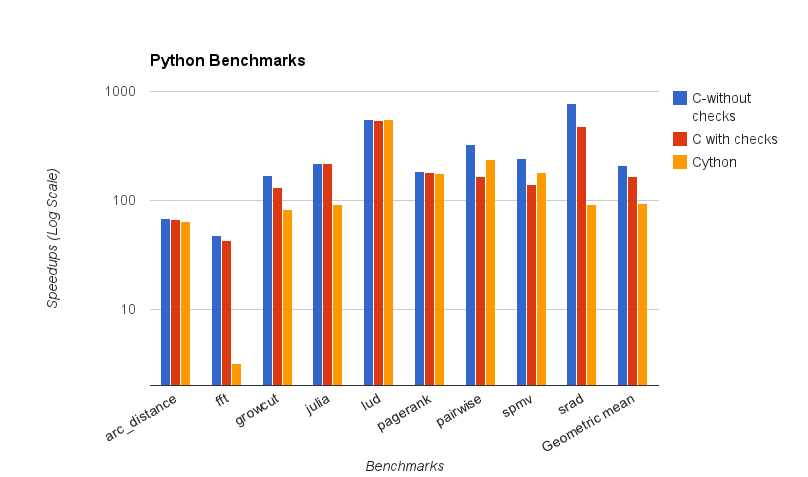
\includegraphics[scale=0.5]{Figures/results_cwochecks_py.png}
\caption{Comparison of the execution times of C backends with and without benchmarks. }
\label{fig:results_cwochecks_py}
\end{figure}
